\documentclass[11pt,]{article}
\usepackage[]{mathpazo}
\usepackage{amssymb,amsmath}
\usepackage{ifxetex,ifluatex}
\usepackage{fixltx2e} % provides \textsubscript
\ifnum 0\ifxetex 1\fi\ifluatex 1\fi=0 % if pdftex
  \usepackage[T1]{fontenc}
  \usepackage[utf8]{inputenc}
\else % if luatex or xelatex
  \ifxetex
    \usepackage{mathspec}
  \else
    \usepackage{fontspec}
  \fi
  \defaultfontfeatures{Ligatures=TeX,Scale=MatchLowercase}
\fi
% use upquote if available, for straight quotes in verbatim environments
\IfFileExists{upquote.sty}{\usepackage{upquote}}{}
% use microtype if available
\IfFileExists{microtype.sty}{%
\usepackage{microtype}
\UseMicrotypeSet[protrusion]{basicmath} % disable protrusion for tt fonts
}{}
\usepackage[margin=1in]{geometry}
\usepackage{hyperref}
\hypersetup{unicode=true,
            pdftitle={Case Study: Predicting the outcomes of the 2017 Dutch General Elections},
            pdfauthor={Ilse van Beelen, Floor Komen},
            pdfkeywords={put some keywords here},
            pdfborder={0 0 0},
            breaklinks=true}
\urlstyle{same}  % don't use monospace font for urls
\usepackage{natbib}
\bibliographystyle{plainnat}
\usepackage{color}
\usepackage{fancyvrb}
\newcommand{\VerbBar}{|}
\newcommand{\VERB}{\Verb[commandchars=\\\{\}]}
\DefineVerbatimEnvironment{Highlighting}{Verbatim}{commandchars=\\\{\}}
% Add ',fontsize=\small' for more characters per line
\usepackage{framed}
\definecolor{shadecolor}{RGB}{248,248,248}
\newenvironment{Shaded}{\begin{snugshade}}{\end{snugshade}}
\newcommand{\KeywordTok}[1]{\textcolor[rgb]{0.13,0.29,0.53}{\textbf{#1}}}
\newcommand{\DataTypeTok}[1]{\textcolor[rgb]{0.13,0.29,0.53}{#1}}
\newcommand{\DecValTok}[1]{\textcolor[rgb]{0.00,0.00,0.81}{#1}}
\newcommand{\BaseNTok}[1]{\textcolor[rgb]{0.00,0.00,0.81}{#1}}
\newcommand{\FloatTok}[1]{\textcolor[rgb]{0.00,0.00,0.81}{#1}}
\newcommand{\ConstantTok}[1]{\textcolor[rgb]{0.00,0.00,0.00}{#1}}
\newcommand{\CharTok}[1]{\textcolor[rgb]{0.31,0.60,0.02}{#1}}
\newcommand{\SpecialCharTok}[1]{\textcolor[rgb]{0.00,0.00,0.00}{#1}}
\newcommand{\StringTok}[1]{\textcolor[rgb]{0.31,0.60,0.02}{#1}}
\newcommand{\VerbatimStringTok}[1]{\textcolor[rgb]{0.31,0.60,0.02}{#1}}
\newcommand{\SpecialStringTok}[1]{\textcolor[rgb]{0.31,0.60,0.02}{#1}}
\newcommand{\ImportTok}[1]{#1}
\newcommand{\CommentTok}[1]{\textcolor[rgb]{0.56,0.35,0.01}{\textit{#1}}}
\newcommand{\DocumentationTok}[1]{\textcolor[rgb]{0.56,0.35,0.01}{\textbf{\textit{#1}}}}
\newcommand{\AnnotationTok}[1]{\textcolor[rgb]{0.56,0.35,0.01}{\textbf{\textit{#1}}}}
\newcommand{\CommentVarTok}[1]{\textcolor[rgb]{0.56,0.35,0.01}{\textbf{\textit{#1}}}}
\newcommand{\OtherTok}[1]{\textcolor[rgb]{0.56,0.35,0.01}{#1}}
\newcommand{\FunctionTok}[1]{\textcolor[rgb]{0.00,0.00,0.00}{#1}}
\newcommand{\VariableTok}[1]{\textcolor[rgb]{0.00,0.00,0.00}{#1}}
\newcommand{\ControlFlowTok}[1]{\textcolor[rgb]{0.13,0.29,0.53}{\textbf{#1}}}
\newcommand{\OperatorTok}[1]{\textcolor[rgb]{0.81,0.36,0.00}{\textbf{#1}}}
\newcommand{\BuiltInTok}[1]{#1}
\newcommand{\ExtensionTok}[1]{#1}
\newcommand{\PreprocessorTok}[1]{\textcolor[rgb]{0.56,0.35,0.01}{\textit{#1}}}
\newcommand{\AttributeTok}[1]{\textcolor[rgb]{0.77,0.63,0.00}{#1}}
\newcommand{\RegionMarkerTok}[1]{#1}
\newcommand{\InformationTok}[1]{\textcolor[rgb]{0.56,0.35,0.01}{\textbf{\textit{#1}}}}
\newcommand{\WarningTok}[1]{\textcolor[rgb]{0.56,0.35,0.01}{\textbf{\textit{#1}}}}
\newcommand{\AlertTok}[1]{\textcolor[rgb]{0.94,0.16,0.16}{#1}}
\newcommand{\ErrorTok}[1]{\textcolor[rgb]{0.64,0.00,0.00}{\textbf{#1}}}
\newcommand{\NormalTok}[1]{#1}
\usepackage{graphicx,grffile}
\makeatletter
\def\maxwidth{\ifdim\Gin@nat@width>\linewidth\linewidth\else\Gin@nat@width\fi}
\def\maxheight{\ifdim\Gin@nat@height>\textheight\textheight\else\Gin@nat@height\fi}
\makeatother
% Scale images if necessary, so that they will not overflow the page
% margins by default, and it is still possible to overwrite the defaults
% using explicit options in \includegraphics[width, height, ...]{}
\setkeys{Gin}{width=\maxwidth,height=\maxheight,keepaspectratio}
\IfFileExists{parskip.sty}{%
\usepackage{parskip}
}{% else
\setlength{\parindent}{0pt}
\setlength{\parskip}{6pt plus 2pt minus 1pt}
}
\setlength{\emergencystretch}{3em}  % prevent overfull lines
\providecommand{\tightlist}{%
  \setlength{\itemsep}{0pt}\setlength{\parskip}{0pt}}
\setcounter{secnumdepth}{0}
% Redefines (sub)paragraphs to behave more like sections
\ifx\paragraph\undefined\else
\let\oldparagraph\paragraph
\renewcommand{\paragraph}[1]{\oldparagraph{#1}\mbox{}}
\fi
\ifx\subparagraph\undefined\else
\let\oldsubparagraph\subparagraph
\renewcommand{\subparagraph}[1]{\oldsubparagraph{#1}\mbox{}}
\fi

%%% Use protect on footnotes to avoid problems with footnotes in titles
\let\rmarkdownfootnote\footnote%
\def\footnote{\protect\rmarkdownfootnote}

%%% Change title format to be more compact
\usepackage{titling}

% Create subtitle command for use in maketitle
\newcommand{\subtitle}[1]{
  \posttitle{
    \begin{center}\large#1\end{center}
    }
}

\setlength{\droptitle}{-2em}

  \title{Case Study: Predicting the outcomes of the 2017 Dutch General Elections}
    \pretitle{\vspace{\droptitle}\centering\huge}
  \posttitle{\par}
    \author{Ilse van Beelen, Floor Komen}
    \preauthor{\centering\large\emph}
  \postauthor{\par}
      \predate{\centering\large\emph}
  \postdate{\par}
    \date{January 20, 2019}

\usepackage{float}

\begin{document}
\maketitle
\begin{abstract}
Put the abstract over here
\end{abstract}

\section{Abstract}\label{abstract}

For this report demographics of Dutch municipalities are compared with
the results of the general Dutch election of 2017. The demographic
variables are the \emph{Urban index}, the \emph{fraction of highly
educated residents}, \emph{Mean income}, \emph{fraction of 60 plus
residents} in a municipality and the factor \emph{Non western}. This
factor devides municipalities in the once with less than 5\%, 5-10\% and
more than 10\% Non-western residents.

This research focusses on the results for party CDA. The goal is to find
voting trends per demographic group and to make future predictions for
CDA. This goal is approached with two different models. The first is a
linear model with a log transformation of the respons. The cross
validation resulted in a Mean Squared Error (MSE) of 0.058. The second,
is a binomial model with the logit as link function. The found MSE is
0.0017.

It is difficult to say which model fits the data better, because they
have different significant variables. Furthermore both have their
limitations and the data showed a large overdispersion. It is not likely
that predictions for future elections can be made with these models.

\section{1. Introduction}\label{introduction}

\subsection{1.1 Motivation}\label{motivation}

For this case study, it was decided to combine the outcome from the
Dutch elections of 2017 and demographic data. Both are collected per
municipality and are well maintained and reliable. This will hopefully
result in observing voting trends per demographic group. The final goal
is to validate the model for making future predictions.

\begin{figure}
\centering
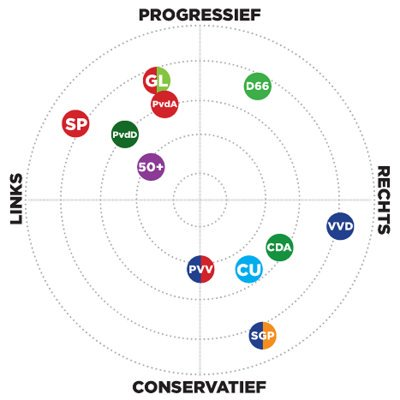
\includegraphics[width=2.60417in]{Partijlandschap.jpg}
\caption{Party landscape}
\end{figure}

\textbf{Dutch political parties}\\
This figure displays the diffences between the political parties in the
Netherlands. The Netherlands has a total of 13 parties. This
investigation focusses on only one party. This party should not be to
extreme left/right/conservative/progressive and should also be one of
the bigger parties. Otherwise, there is not enough data available,
making the results less reliable. Therefore, party CDA is chosen.

In this research the above described demographics are chosen because of
their influence on a municipality level. The expectation is that a
municipality with more non-western residents for example votes different
than a municipality with less non-western residents. This is the same
for the other two demographics. Other demographics are also researched,
for example gender, but on a municipality level there is no large
difference between the amount of men and women per municipality. So that
is a more interesting demographic to research on an individual level.
\emph{The standardized income per municipality} are given in thousands.
\emph{Urban index} of a municipality is a database with five categories
per municipality. These five categories are:

\begin{itemize}
\item 0. No urbanity (less than 500 addresses per $km^2$)
\item 1. Little urbanity (500-1000 addresses per $km^2$)
\item 2. Moderate urbanity (1000- 1500 addresses per $km^2$)
\item 3. Strong urbanity (1500-2500 addresses per $km^2$) 
\item 4. Really strong urbanity (more than 2500 addresses per $km^2$)
\end{itemize}

Per municipality the amount of \(km^2\) per category is given. The
\emph{non-west residents per municipality} is given as an amount per
municipality, also the total amount of residents is given per
municipality.

\subsection{1.2 Data sources}\label{data-sources}

\textbf{Electoral data} For the electoral data, the results of the 2017
general election are used. This is the most recent national election and
is of the most important election type in the Netherlands. Furthermore,
it had a turnup of 81.9\%. Therefore, it seems plausible that the data
for this election is representative of the political makeup of different
municipalities. We downloaded the raw data directly from the official
government source.\footnote{\url{https://data.overheid.nl/data/dataset/verkiezingsuitslag-tweede-kamer-2017}}
This contained a .csv file with the raw number of votes for every party
in every municipality.

\textbf{Demographical data}\\
We got our demographical data from the CBS, the official Dutch
statistical agency.\footnote{\url{https://opendata.cbs.nl/statline/\#/CBS/nl/dataset/70072ned/table?ts=1544803364892}}
From the wealth of demographical information available we picked a
handful of attributes that we suspected (based on prior research and
some gut feeling) to be useful as predictor variables. We landed on five
demographical attributes: education grade, average income, age,
urbanization and the amount of people with a non-western background.
Note that the data we downloaded from the CBS site usually had to be
transformed to get it in a useful predictor variable format. The
specifics of these are described in the next section.

\subsection{1.3 Data cleaning}\label{data-cleaning}

An extensive amount of data cleaning had to be done. Below these steps
are describes and a small part of code is displayed.

\textbf{Electoral data}

\textbf{Demographical data}

The variable \emph{non-western residents} are divided in three groups:

\begin{itemize}
\item Municipalities with less than 5 % non-western residents 
\item Municipalities with 5-10 % non-western resident 
\item Municipalities with mre than 10 % non-western residents
\end{itemize}

\begin{Shaded}
\begin{Highlighting}[]
\NormalTok{Data_CDA}\OperatorTok{$}\NormalTok{Non_west <-}\StringTok{ }\KeywordTok{ifelse}\NormalTok{(Data_CDA}\OperatorTok{$}\NormalTok{Non_west_frac }\OperatorTok{<}\StringTok{ }\FloatTok{0.05}\NormalTok{, }\DecValTok{1}\NormalTok{, }\OtherTok{NA}\NormalTok{)}
\NormalTok{Data_CDA}\OperatorTok{$}\NormalTok{Non_west <-}\StringTok{ }\KeywordTok{ifelse}\NormalTok{(Data_CDA}\OperatorTok{$}\NormalTok{Non_west_frac }\OperatorTok{>=}\StringTok{ }\FloatTok{0.05} \OperatorTok{&}\StringTok{ }\NormalTok{Data_CDA}\OperatorTok{$}\NormalTok{Non_west_frac }\OperatorTok{<}\StringTok{ }
\StringTok{    }\FloatTok{0.1}\NormalTok{, }\DecValTok{2}\NormalTok{, Data_CDA}\OperatorTok{$}\NormalTok{Non_west)}
\NormalTok{Data_CDA}\OperatorTok{$}\NormalTok{Non_west <-}\StringTok{ }\KeywordTok{ifelse}\NormalTok{(Data_CDA}\OperatorTok{$}\NormalTok{Non_west_frac }\OperatorTok{>=}\StringTok{ }\FloatTok{0.1}\NormalTok{, }\DecValTok{3}\NormalTok{, Data_CDA}\OperatorTok{$}\NormalTok{Non_west)}
\NormalTok{Data_CDA}\OperatorTok{$}\NormalTok{Non_west <-}\StringTok{ }\KeywordTok{as.factor}\NormalTok{(Data_CDA}\OperatorTok{$}\NormalTok{Non_west)}
\end{Highlighting}
\end{Shaded}

At last, the electoral data and demographic data are combined again.
Only the municipality Boxmeer is removed, due to a mistake not all the
votes are reported here\footnote{\url{https://www.gelderlander.nl/boxmeer/7-600-stemmen-in-boxmeer-niet-meegenomen-in-uitslag-verkiezingen~a063ee9e/}}.
The final dataset has no NAs

\begin{Shaded}
\begin{Highlighting}[]
\KeywordTok{summary}\NormalTok{(Data_CDA)}
\end{Highlighting}
\end{Shaded}

\begin{verbatim}
##      Muni              CDA_frac       Urban_index     High_educated_frac
##  Length:366         Min.   :0.0310   Min.   :0.0000   Min.   :0.1200    
##  Class :character   1st Qu.:0.1170   1st Qu.:0.6623   1st Qu.:0.2200    
##  Mode  :character   Median :0.1420   Median :1.2305   Median :0.2600    
##                     Mean   :0.1528   Mean   :1.4280   Mean   :0.2662    
##                     3rd Qu.:0.1820   3rd Qu.:2.1750   3rd Qu.:0.3000    
##                     Max.   :0.4200   Max.   :3.7890   Max.   :0.4700    
##   Mean_income    Non_west_frac        CDA_abs        Total_abs     
##  Min.   :20.80   Min.   :0.01000   Min.   :  421   Min.   :  2727  
##  1st Qu.:24.30   1st Qu.:0.03000   1st Qu.: 1737   1st Qu.: 11516  
##  Median :25.60   Median :0.05000   Median : 2510   Median : 16915  
##  Mean   :25.91   Mean   :0.06574   Mean   : 3254   Mean   : 25162  
##  3rd Qu.:27.00   3rd Qu.:0.08000   3rd Qu.: 4023   3rd Qu.: 27087  
##  Max.   :41.80   Max.   :0.38000   Max.   :18813   Max.   :440854  
##   Frac_60plus     Non_west
##  Min.   :0.0700   1:178   
##  1st Qu.:0.1200   2:111   
##  Median :0.1300   3: 77   
##  Mean   :0.1327           
##  3rd Qu.:0.1400           
##  Max.   :0.1800
\end{verbatim}

\subsection{1.3 Data visualisation}\label{data-visualisation}

In this part the cleaned data is visualized, so that a good picture can
be obtained of the current data. First of all some demographics of data
will be showed. In figure \ref{1} of the \emph{parties}, \emph{the urban
index}, \emph{the percentage of highly educated residents}, \emph{the
mean income}, \emph{The non west residents factor} and * the percentage
60 plus* are plotted. As you can see in the plot, they are normal
distributed. Because of the low values at the x-axis, the CDA,
GroenLinks, 60 plus percentage and the highly educated densities are
above 1. The area beneath the curve sums to 1, so it is correct.

\begin{figure}[H]

{\centering 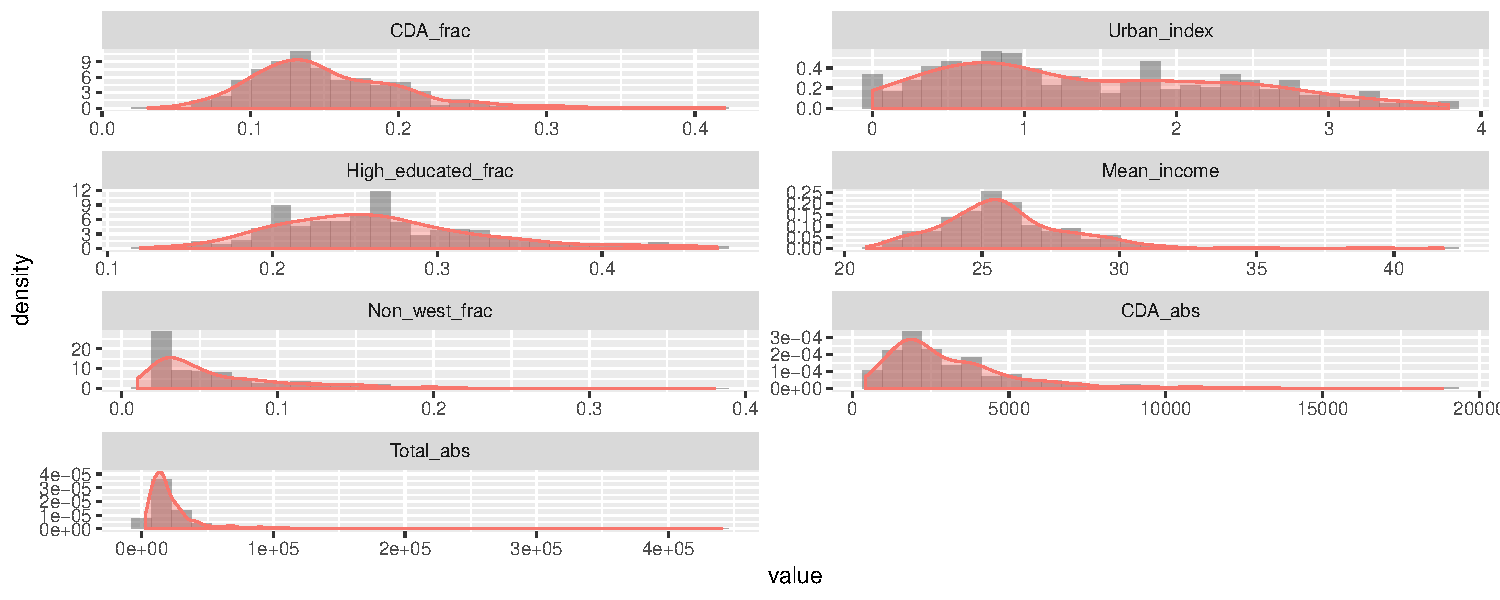
\includegraphics{Report_files/figure-latex/demographics_data-1} 

}

\caption{\label{1} Density plot}\label{fig:demographics_data}
\end{figure}

\textbf{Correlation heatmap} In this heatmap (figure \ref{2}) the
correlation between explanatory and respons variable are showed. The red
color means a positive relation, the purple color means a negative
relation. The non\_west variable is not taken into account, because it
is a factor and the other variables are continous.

\begin{figure}[H]

{\centering 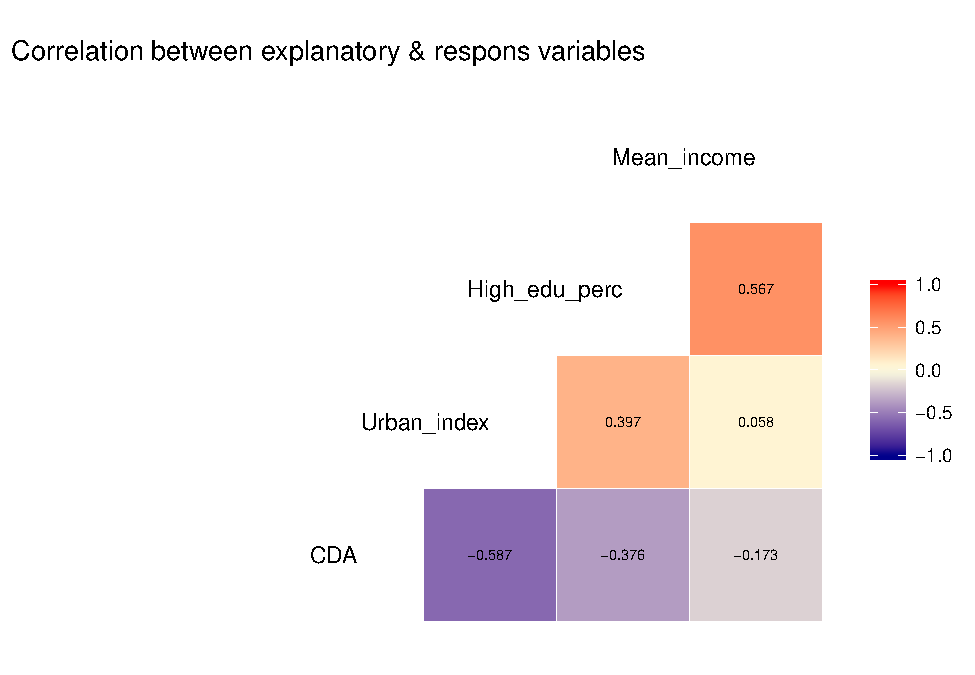
\includegraphics{Report_files/figure-latex/correlation_heatmap-1} 

}

\caption{\label{2}Correlation between explanatory and respons variables}\label{fig:correlation_heatmap}
\end{figure}

\textbf{Multilineair plots CDA } In these two plots you can see a
scatterplot with on the y-axis the votes for CDA in percentages and on
the x-axis on the left graph the mean income per municipality in 1000
euro. The right plot has the urbanity index as x-axis. As you can see,
the trend is that when the mean income goes up, the votes for CDA goes
down. Same with the urbanity index. In the model formulation graph these
trends are checked.

\begin{figure}[H]

{\centering 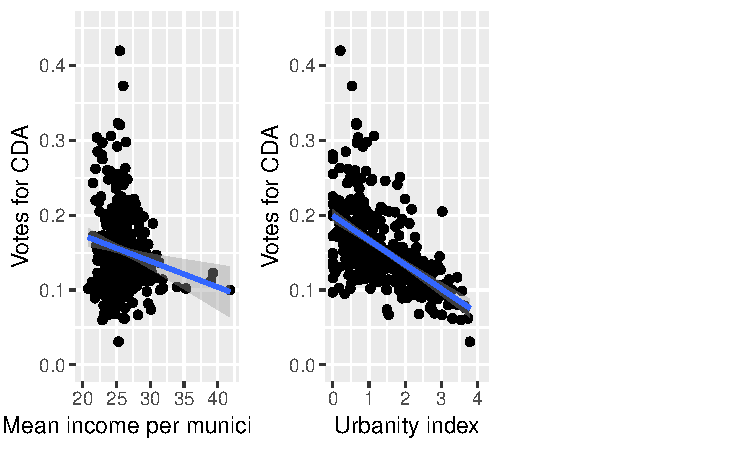
\includegraphics{Report_files/figure-latex/unnamed-chunk-6-1} 

}

\caption{\label{3}Scatterplots CDA}\label{fig:unnamed-chunk-6}
\end{figure}

\textbf{Exploratory plots of variables} These three plots are
scatterplots of the explanatory variables.

\begin{figure}[H]

{\centering 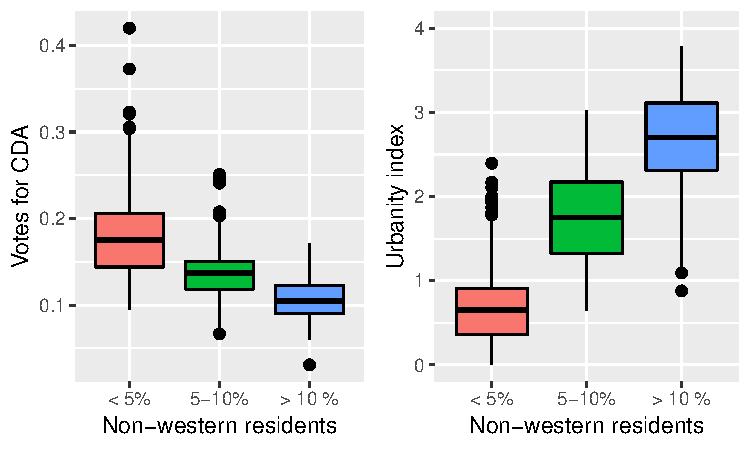
\includegraphics{Report_files/figure-latex/unnamed-chunk-7-1} 

}

\caption{\label{5}Scatterplot explanatory variables}\label{fig:unnamed-chunk-71}
\end{figure}\begin{figure}[H]

{\centering 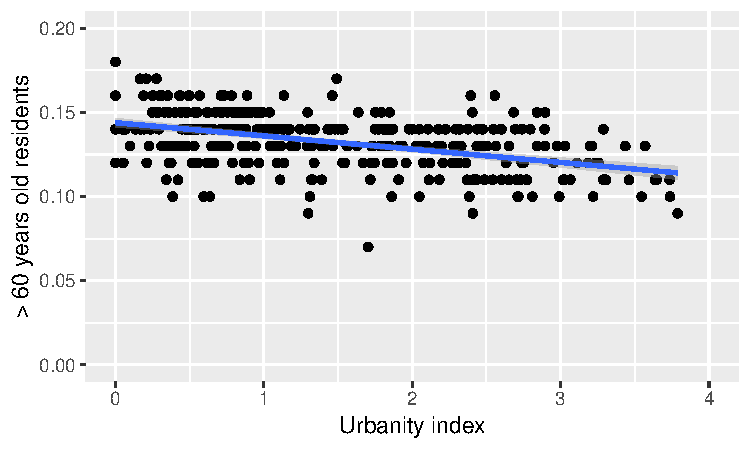
\includegraphics{Report_files/figure-latex/unnamed-chunk-7-2} 

}

\caption{\label{5}Scatterplot explanatory variables}\label{fig:unnamed-chunk-72}
\end{figure}

\textbf{Multiple boxplots} In this graph boxplots are made, to compare
some variables. A boxplot is a standardized way to display the
distribution of data. It gives the minimum, first quartile, median,
third quartile and the maximum. If there are any outliers, the boxplot
is extended with those. The line within the box is the median, the first
and third quartile are the down- and upside of the box, respectively.
The length of the box is the Inter Quartile Range (IQR). The minimum and
maximum are 1.5X Inter Quartile Range (IQR). Observations further away
can be considered outliers.

\begin{figure}[H]

{\centering 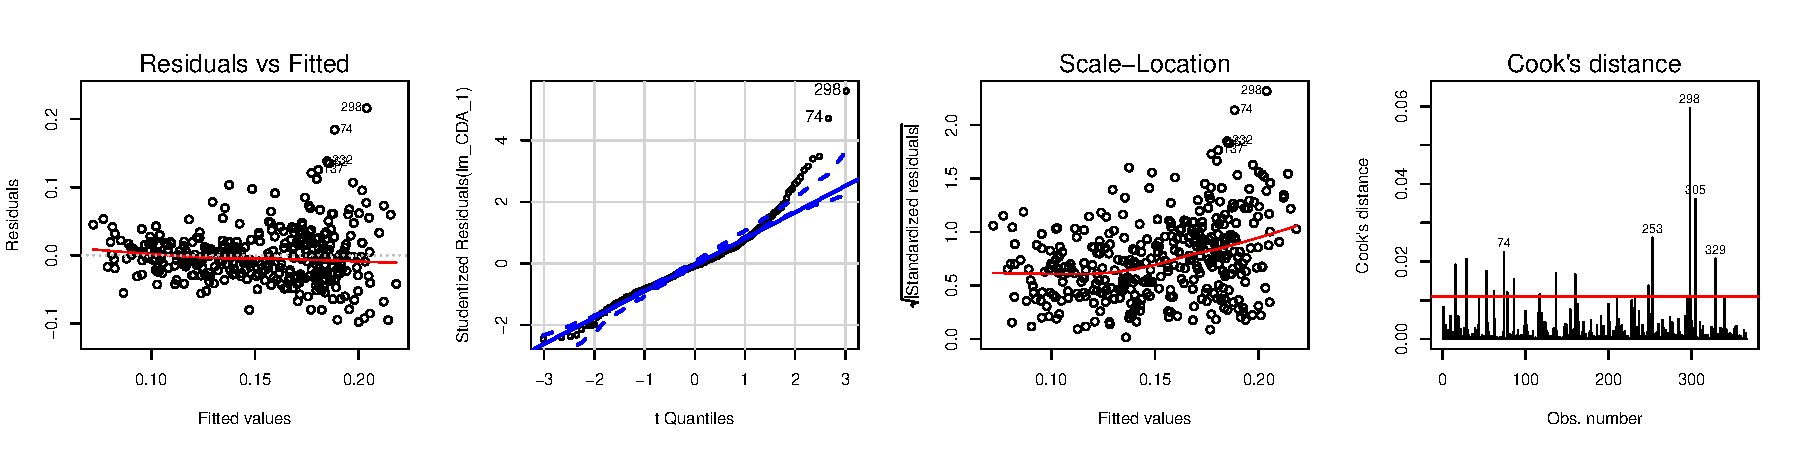
\includegraphics{Report_files/figure-latex/unnamed-chunk-8-1} 

}

\caption{\label{6}Three boxplots: Votes for CDA, Votes for GroenLinks and Urbanity index}\label{fig:unnamed-chunk-8}
\end{figure}

\section{2. Multiple linear
regression}\label{multiple-linear-regression}

In this chapter multiple linear models are generated. The demographics
tested in this model are the highly educated fraction in a municipality
\texttt{High\_educated\_frac}, the urban index of a municipality
\texttt{Urban\_index}, the mean income of the municipality
\texttt{Mean\_income}, the non-west factor \texttt{Non\_west} and the
fraction that is 60 plus in the municipality \texttt{Frac\_60plus}. The
error assumptions are also discussed. This are assumptions made for the
residuals, to check if meet the requirements for correct linear
regressions. These assumptions are: * Linearity: The expected value of
the error is zero * Constant variance: The variance of the error is
constant * Normality: The errors are normally distributed * Indepence:
The observations are sampled indipendently

\subsection{First model}\label{first-model}

The first model will be the model with all the demographics:\\
\(Y_i = \beta_0 + \beta_1*high educated fraction + \beta_2*Urban index + \beta_3*Mean income + \beta_4*Non west2 +\beta_5*Non west3 + \beta_6*Frac 60plus + \epsilon i\)\\
The outcome of this model is shown below:

\begin{table}[ht]
\centering
\begin{tabular}{rrrrr}
  \hline
 & Estimate & Std. Error & t value & Pr() \\ 
  \hline
(Intercept) & 0.3381 & 0.0314 & 10.78 & 0.0000 \\ 
  High\_educated\_frac & -0.0864 & 0.0454 & -1.90 & 0.0576 \\ 
  Urban\_index & -0.0193 & 0.0041 & -4.69 & 0.0000 \\ 
  Mean\_income & -0.0015 & 0.0011 & -1.46 & 0.1453 \\ 
  Non\_west2 & -0.0223 & 0.0065 & -3.45 & 0.0006 \\ 
  Non\_west3 & -0.0455 & 0.0095 & -4.77 & 0.0000 \\ 
  Frac\_60plus & -0.5904 & 0.1494 & -3.95 & 0.0001 \\ 
   \hline
\end{tabular}
\end{table}

The first model is the total model, \texttt{high\_educated\_frac} and
\texttt{Mean\_income} do not have a significant t-value. Before any
conclusions are made, the assumptions are checked via plots and the VIF
is checked. The VIF is the Variation Inflation Factor, it implies if
there is multicollinearity between two or more variables. The formula
for VIF is \(1/(1-R^2)\) and the thresholdvalue is 10. So values above
10 give signs of multicollinearity. As shown below none of the values
are above 10, so no signs of collinearity.

\begin{verbatim}
## High_educated_frac        Urban_index        Mean_income 
##           1.871032           3.383149           1.658015 
##          Non_west2          Non_west3        Frac_60plus 
##           1.974537           3.361734           1.289979
\end{verbatim}

\begin{verbatim}
## [1]  74 298
\end{verbatim}

\begin{figure}[H]

{\centering 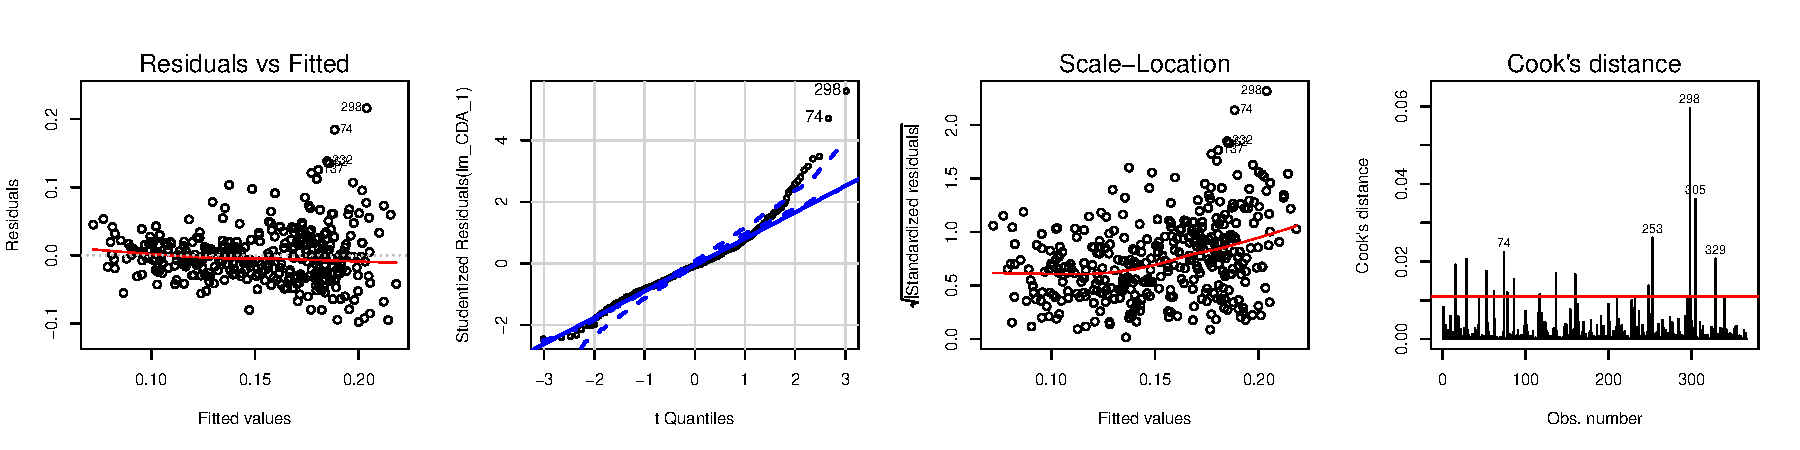
\includegraphics{Report_files/figure-latex/unnamed-chunk-9-1} 

}

\caption{\label{afm}assumptions first model}\label{fig:unnamed-chunk-9}
\end{figure}

In figure \ref{afm} the four plots are shown. The first plot (Residuals
vs Fitted) shows that the residuals have a `loudspeaker pattern', the
variance of the residuals tends to increase with an increase of the
fitted value. Because of this, a BoxCox graph is consulted. This graph
suggests a transformation for the response. The BoxCos figure \ref{BC1}
in has a 95\% Confidence interval located around the 0. So a ln
transformation is suggested.

\begin{figure}[H]

{\centering 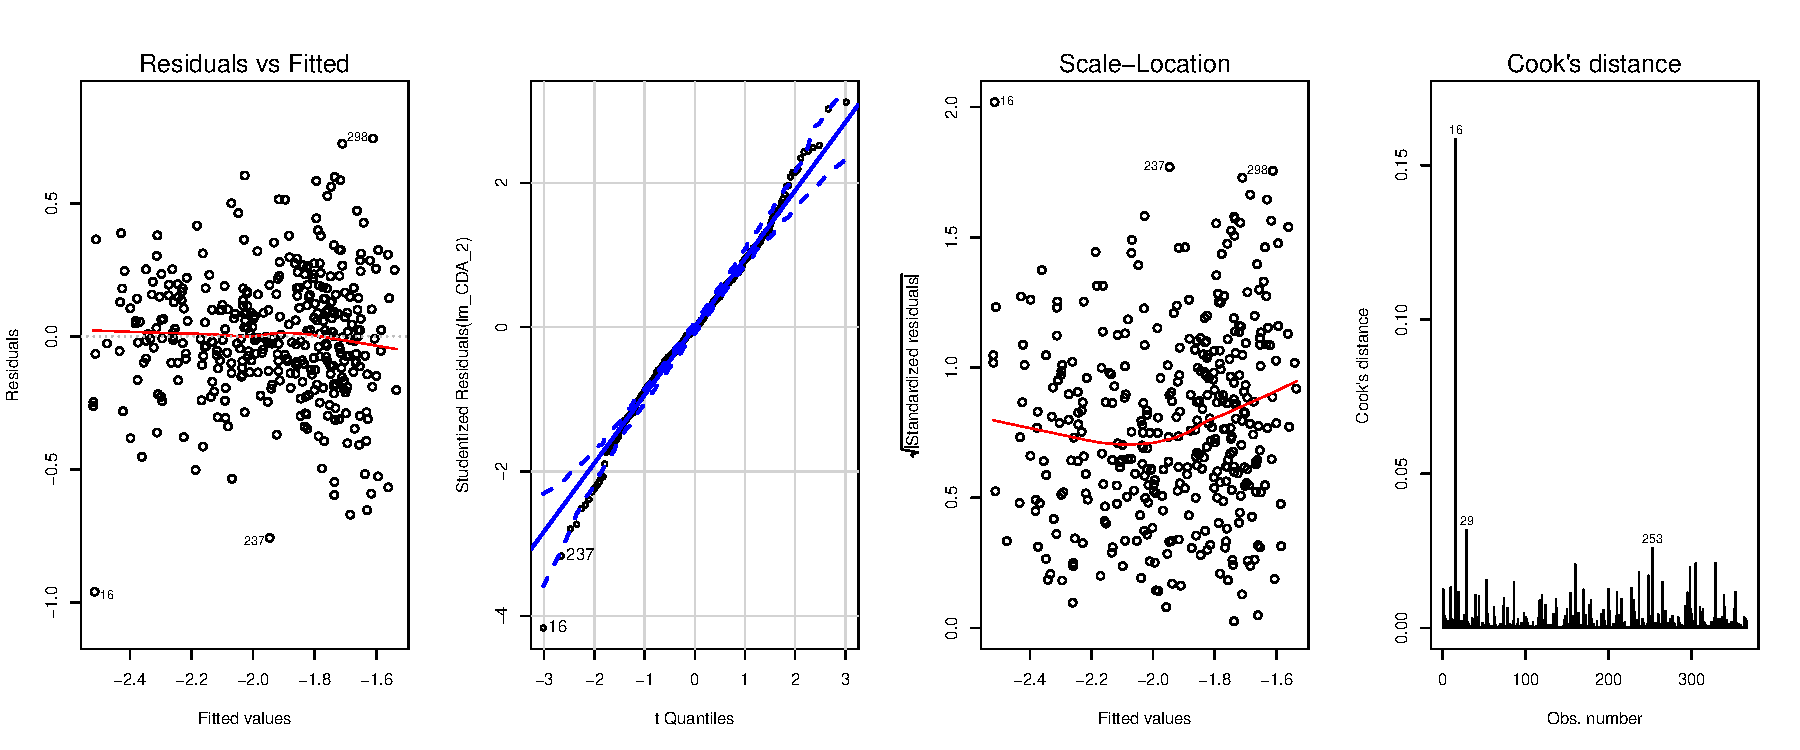
\includegraphics{Report_files/figure-latex/unnamed-chunk-10-1} 

}

\caption{\label{BC1}BoxCox first model}\label{fig:unnamed-chunk-10}
\end{figure}

\subsection{Second model}\label{second-model}

In the second model the response variable will be ln transformed. So the
new model will be:\\
\(ln(Y_i) = \beta_0 + \beta_1*high educated fraction + \beta_2*Urban index + \beta_3*Mean income + \beta_4*Non west2 + \beta_5*Non west 3 + \beta_6*Frac 60plus + \epsilon i\)

\begin{table}[ht]
\centering
\begin{tabular}{rrrrr}
  \hline
 & Estimate & Std. Error & t value & Pr() \\ 
  \hline
(Intercept) & -0.9944 & 0.1882 & -5.28 & 0.0000 \\ 
  High\_educated\_frac & -0.8808 & 0.2723 & -3.24 & 0.0013 \\ 
  Urban\_index & -0.1388 & 0.0247 & -5.62 & 0.0000 \\ 
  Mean\_income & -0.0024 & 0.0064 & -0.38 & 0.7042 \\ 
  Non\_west2 & -0.0991 & 0.0389 & -2.55 & 0.0112 \\ 
  Non\_west3 & -0.2763 & 0.0572 & -4.83 & 0.0000 \\ 
  Frac\_60plus & -2.6940 & 0.8965 & -3.01 & 0.0028 \\ 
   \hline
\end{tabular}
\end{table}

\begin{verbatim}
## [1]  16 237
\end{verbatim}

\begin{figure}[H]

{\centering 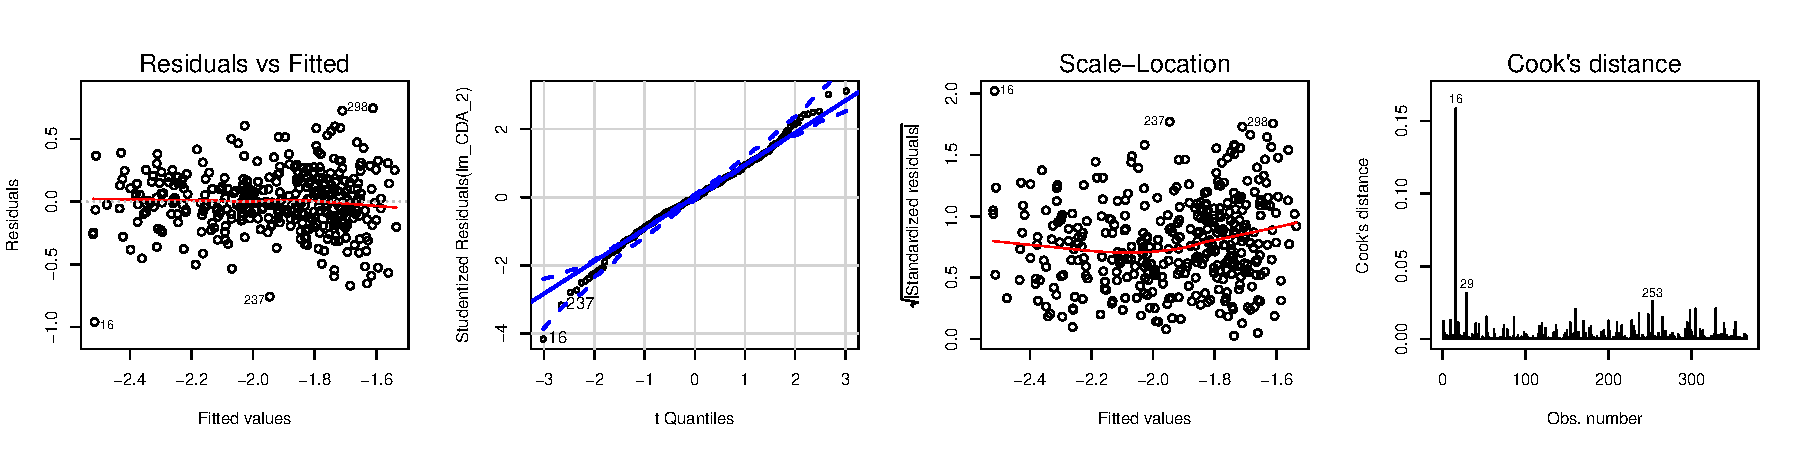
\includegraphics{Report_files/figure-latex/unnamed-chunk-11-1} 

}

\caption{\label{asm}assumptions second model}\label{fig:unnamed-chunk-11}
\end{figure}

The plots in figure \ref{asm} show one big outlier, the municipality
Amsterdam which has number 16. Amsterdams value for the cooks distance
goes way above the cutoff value for cooks, \(4/(369-5-1)=0.011\). It is
also outside the (-3,3) range with the studentized residuals. That is
why this municipality is removed.\\
For the second model without Amsterdam, a step function is used. This
step function uses the AIC for backward elimination. If the AIC can get
lower, because a variable is removed that variable will be removed else
no variable is removed. The formula for AIC is
\(AIC=-2log(likelihood)+2p\), p is the number of parameters in the
model. The variables that are left are the variables used in the final
model.

\begin{verbatim}
## Start:  AIC=-1041.5
## log(CDA_frac) ~ High_educated_frac + Urban_index + Mean_income + 
##     Non_west + Frac_60plus
## 
##                      Df Sum of Sq    RSS     AIC
## - Mean_income         1   0.04208 20.291 -1042.7
## <none>                            20.249 -1041.5
## - High_educated_frac  1   0.36195 20.611 -1037.0
## - Frac_60plus         1   0.67266 20.922 -1031.6
## - Non_west            2   1.54236 21.792 -1018.7
## - Urban_index         1   1.72696 21.976 -1013.6
## 
## Step:  AIC=-1042.74
## log(CDA_frac) ~ High_educated_frac + Urban_index + Non_west + 
##     Frac_60plus
## 
##                      Df Sum of Sq    RSS     AIC
## <none>                            20.291 -1042.7
## - Frac_60plus         1   0.66435 20.956 -1033.0
## - High_educated_frac  1   0.85427 21.146 -1029.7
## - Non_west            2   1.51164 21.803 -1020.5
## - Urban_index         1   1.68687 21.978 -1015.6
\end{verbatim}

\begin{verbatim}
## 
## Call:
## lm(formula = log(CDA_frac) ~ High_educated_frac + Urban_index + 
##     Non_west + Frac_60plus, data = Data_CDA[-16, ])
## 
## Coefficients:
##        (Intercept)  High_educated_frac         Urban_index  
##            -1.0298             -0.8277             -0.1311  
##          Non_west2           Non_west3         Frac_60plus  
##            -0.1141             -0.2871             -3.0168
\end{verbatim}

\subsection{Final model}\label{final-model}

The backward elimination resulted in the final model.\\
\(ln(Y_i) = \beta_0 + \beta_1*high educated fraction + \beta_2*Urban index + \beta_4*Non west2 + \beta_5*Non west 3 + \beta_6*Frac 60plus + \epsilon_i\)
The coëfficients are given in the table below

\begin{table}[ht]
\centering
\begin{tabular}{rrrrr}
  \hline
 & Estimate & Std. Error & t value & Pr($>$$|$t$|$) \\ 
  \hline
(Intercept) & -1.0298 & 0.1365 & -7.54 & 0.0000 \\ 
  High\_educated\_frac & -0.8277 & 0.2129 & -3.89 & 0.0001 \\ 
  Urban\_index & -0.1311 & 0.0240 & -5.46 & 0.0000 \\ 
  Non\_west2 & -0.1141 & 0.0378 & -3.02 & 0.0027 \\ 
  Non\_west3 & -0.2871 & 0.0559 & -5.13 & 0.0000 \\ 
  Frac\_60plus & -3.0168 & 0.8799 & -3.43 & 0.0007 \\ 
   \hline
\end{tabular}
\end{table}

\begin{verbatim}
## 237 298 
## 236 297
\end{verbatim}

\begin{figure}[H]

{\centering 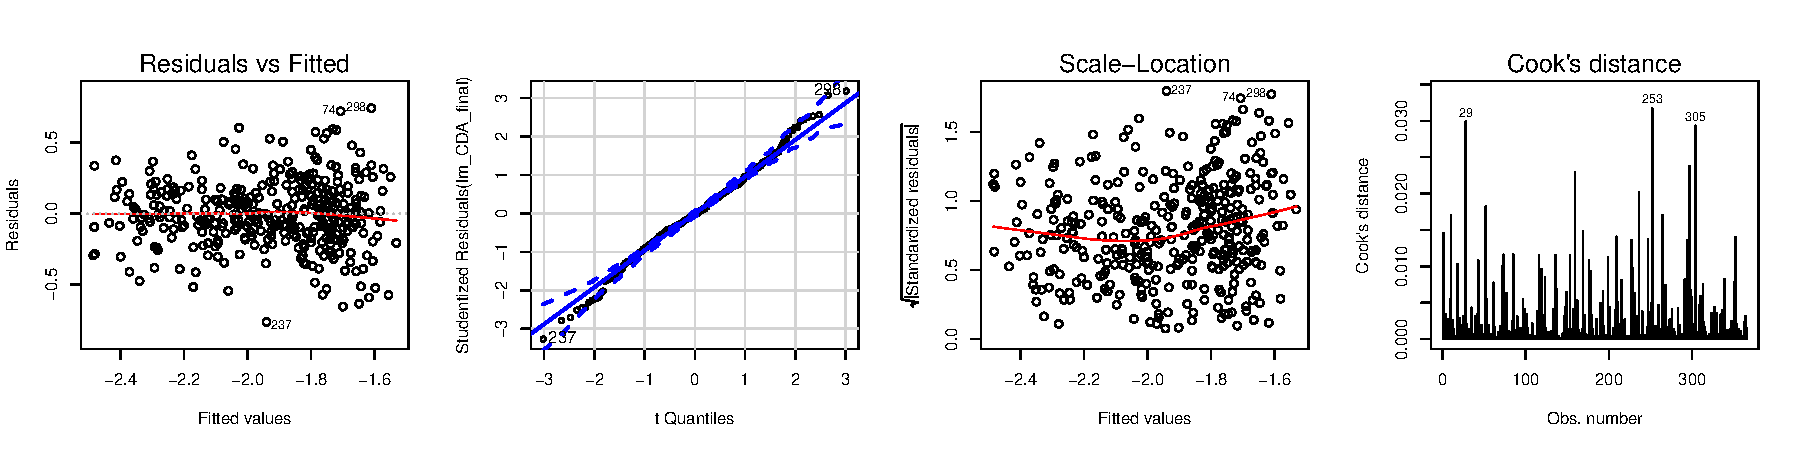
\includegraphics{Report_files/figure-latex/unnamed-chunk-13-1} 

}

\caption{\label{asm}assumptions second model}\label{fig:unnamed-chunk-13}
\end{figure}

The estimates for the predictors are filled in the model and the
following results are obtained:

\(ln(Y_i) = -1.0298 -0.8277*high educated fraction -0.1311*Urban index -0.1141*Non west2 -0.2871*Non west3 -3.0168*Frac 60plus + \epsilon i\)

All the coëfficients are negative, but because the fitted value is a log
value it will be positive.

\subsection{Cross validation}\label{cross-validation}

To tell something about the prediction possibilities of the model, cross
validation is done. Cross validation tells something about how well the
model predicts on average, it telss nothing about the 'correctness'of
the model. Cross validation estimates the expected prediction error of a
model.\\
The cross validation works as follows. First 5k-folds are made. This
means that the data is divided in five folds. Next, the loss function is
made. This function makes the square of the real value minues the
predicted value. By taking the sum of these values and the deviation by
amount of real values in the k-folds, the mean is taken. 4 of the 5
kfolds are used ase training data, the other one is the test/validation
data. The model is fitted on the training data and afterwards it tries
to fit on the test data, to see if it predicts closely. This is done 5
times, every time another fold is is the testdata. As is shown below,
the prediction error for this model is 0.0582

\begin{Shaded}
\begin{Highlighting}[]
\NormalTok{lm_CDA_final <-}\StringTok{ }\KeywordTok{lm}\NormalTok{(}\KeywordTok{log}\NormalTok{(CDA_frac) }\OperatorTok{~}\StringTok{ }\NormalTok{High_educated_frac }\OperatorTok{+}\StringTok{ }\NormalTok{Urban_index }\OperatorTok{+}\StringTok{ }\NormalTok{Non_west }\OperatorTok{+}\StringTok{ }
\StringTok{    }\NormalTok{Frac_60plus, }\DataTypeTok{data =}\NormalTok{ Data_CDA[}\OperatorTok{-}\DecValTok{16}\NormalTok{, ])}
\NormalTok{K <-}\StringTok{ }\DecValTok{5}
\NormalTok{index <-}\StringTok{ }\KeywordTok{rep}\NormalTok{(}\DecValTok{1}\OperatorTok{:}\NormalTok{K, }\KeywordTok{floor}\NormalTok{(}\KeywordTok{nrow}\NormalTok{(Data_CDA)}\OperatorTok{/}\NormalTok{K) }\OperatorTok{+}\StringTok{ }\DecValTok{1}\NormalTok{)[}\DecValTok{1}\OperatorTok{:}\KeywordTok{nrow}\NormalTok{(Data_CDA)]}
\NormalTok{fold.index <-}\StringTok{ }\KeywordTok{sample}\NormalTok{(index)}
\NormalTok{Loss <-}\StringTok{ }\ControlFlowTok{function}\NormalTok{(x, y) \{}
    \KeywordTok{sum}\NormalTok{((x }\OperatorTok{-}\StringTok{ }\NormalTok{y)}\OperatorTok{^}\DecValTok{2}\NormalTok{)}\OperatorTok{/}\KeywordTok{length}\NormalTok{(x)}
\NormalTok{\}}
\NormalTok{loss <-}\StringTok{ }\KeywordTok{numeric}\NormalTok{(K)}
\ControlFlowTok{for}\NormalTok{ (k }\ControlFlowTok{in} \DecValTok{1}\OperatorTok{:}\NormalTok{K) \{}
\NormalTok{    training <-}\StringTok{ }\NormalTok{Data_CDA[fold.index }\OperatorTok{!=}\StringTok{ }\NormalTok{k, ]}
\NormalTok{    validation <-}\StringTok{ }\NormalTok{Data_CDA[fold.index }\OperatorTok{==}\StringTok{ }\NormalTok{k, ]}
\NormalTok{    training.fit <-}\StringTok{ }\NormalTok{lm_CDA_final}
\NormalTok{    validation.predict <-}\StringTok{ }\KeywordTok{predict}\NormalTok{(training.fit, }\DataTypeTok{newdata =}\NormalTok{ validation, }\DataTypeTok{type =} \StringTok{"response"}\NormalTok{)}
\NormalTok{    loss[k] <-}\StringTok{ }\KeywordTok{Loss}\NormalTok{(}\KeywordTok{log}\NormalTok{(validation}\OperatorTok{$}\NormalTok{CDA_frac), validation.predict)}
\NormalTok{\}}
\KeywordTok{mean}\NormalTok{(loss)}
\end{Highlighting}
\end{Shaded}

\begin{verbatim}
## [1] 0.05813659
\end{verbatim}

\section{3. Logistic regression}\label{logistic-regression}

The raw respons variable is the absolute amount of residents per
municipality that voted for CDA. For linear regresssion, this variable
is transformed to a fraction. However, the absolute total amount of
votes per municipality is also available. Therefore, a binomial model
would be a better fit to the data. A second model is developed that uses
the logit as link function to transform the range of the respons. The
choice for the logit was easily made. Because the inverse of the logit
is directly interpretable as the log-odds ratio and this link displays
the underlaying pattern of the data best. Below, the formula for the
link function:

\(\eta = log(\frac{\theta}{1 - \theta}) = \beta_0 + \beta_1 x_1 + \beta_2 x_2 + ... + \beta_n x_n\)

Where \(\theta\) is the probability of votes for CDA.

Also for logistics regression diagnostic plots are needed to visualise
the deviance/pearson residuals and search for outliers. Most of the
diagnostics from the linear model extend relatively straighforward to
logistic regression. However, leverages are no longer just a function of
the explanatory variable, but also depend on the respons due to the
iterated weighted least squares. Furthermore, \(\theta\) can never be
zero or one. Fortunately, this was not the case for any of the
observations in this dataset.

\subsection{3.1 First model}\label{first-model-1}

Again, the first is the full model. Stepwise backward elimination is
used to find the optimal model. Below, the formula for the full model:

\(log(\frac{\theta_i}{1 - \theta_i}) = \beta_0 + \beta_1 \cdot UrbanIndex + \beta_2 \cdot HighlyEducatedFraction + \beta_3 \cdot MeanIncome + \beta_4 \cdot NonWest + \beta_5 \cdot Fraction60Plus + \epsilon_i\)

With \(i = 1, 2,.., N\) for the number of observations.

Below the summary of this model:

\begin{table}[ht]
\centering
\begin{tabular}{rrrrr}
  \hline
 & Estimate & Std. Error & z value & Pr($>$$|$z$|$) \\ 
  \hline
(Intercept) & -1.0560 & 0.0157 & -67.29 & 0.0000 \\ 
  Urban\_index & -0.1934 & 0.0020 & -94.91 & 0.0000 \\ 
  High\_educated\_frac & -2.1028 & 0.0200 & -105.38 & 0.0000 \\ 
  Mean\_income & 0.0156 & 0.0005 & 29.32 & 0.0000 \\ 
  Non\_west2 & -0.0563 & 0.0032 & -17.81 & 0.0000 \\ 
  Non\_west3 & -0.2593 & 0.0046 & -56.26 & 0.0000 \\ 
  Frac\_60plus & -1.3424 & 0.0737 & -18.20 & 0.0000 \\ 
   \hline
\end{tabular}
\end{table}

The summary shows that the all the variables are very significant and
have small standard errors. The full model has 359 degrees of freedom
and it is expected that the residual deviance is roughly equivalent.
However, the residual deviance is far above this value. These are strong
indications that this model suffers from overdispersion. This assumption
seems reasonable, because there is a very large variance in how many
residents per municapality voted for CDA. In some municipalities only
3\% voted for CDA, while it others nearly 50\% voted for CDA. It is
concluded that a quasi-binomial would fit the data better.

\subsection{3.2 Second model}\label{second-model-1}

The second model has still all the variables, but is fitted to a
quasi-binomial. Below the output of the summary is visualized:

\begin{table}[ht]
\centering
\begin{tabular}{rrrrr}
  \hline
 & Estimate & Std. Error & t value & Pr($>$$|$t$|$) \\ 
  \hline
(Intercept) & -1.0560 & 0.2501 & -4.22 & 0.0000 \\ 
  Urban\_index & -0.1934 & 0.0325 & -5.95 & 0.0000 \\ 
  High\_educated\_frac & -2.1028 & 0.3180 & -6.61 & 0.0000 \\ 
  Mean\_income & 0.0156 & 0.0085 & 1.84 & 0.0667 \\ 
  Non\_west2 & -0.0563 & 0.0504 & -1.12 & 0.2647 \\ 
  Non\_west3 & -0.2593 & 0.0735 & -3.53 & 0.0005 \\ 
  Frac\_60plus & -1.3424 & 1.1753 & -1.14 & 0.2541 \\ 
   \hline
\end{tabular}
\end{table}

By applying a quasi binomial model, a dispersion parameter \(\phi\) is
included, resulting in larger standard errors and less significant
p-values. \(\phi\) is estimated on the data at 254.0441. Furthermore,
the null deviance is estimated at 247,550 with 365 df and the residual
at 89969 with 359 df. The variables \texttt{Frac\_60plus},
\texttt{Mean\_income} and factor level \texttt{Non\_west2} are no longer
significant.

No goodness of fit test is possible because of the free dispersion
parameter. The decision to remove variables is done based on the lowest
F-test.

\begin{verbatim}
##        Urban_index High_educated_frac        Mean_income 
##       0.0013605627       0.0005943712       0.0006876039 
##          Non_west2          Non_west3        Frac_60plus 
##       0.0007725368       0.0012914703       0.0005161910
\end{verbatim}

\begin{verbatim}
## Single term deletions
## 
## Model:
## cbind(CDA_abs, Total_abs - CDA_abs) ~ Urban_index + High_educated_frac + 
##     Mean_income + Non_west + Frac_60plus
##                    Df Deviance F value    Pr(>F)    
## <none>                   89969                      
## Urban_index         1    99052 36.2459 4.300e-09 ***
## High_educated_frac  1   101151 44.6196 9.132e-11 ***
## Mean_income         1    90821  3.3987 0.0660730 .  
## Non_west            2    94112  8.2661 0.0003092 ***
## Frac_60plus         1    90300  1.3217 0.2510613    
## ---
## Signif. codes:  0 '***' 0.001 '**' 0.01 '*' 0.05 '.' 0.1 ' ' 1
\end{verbatim}

According to the F-test \texttt{Frac\_60plus} should be removed. This
variable has a F-value of 1.32 and a corresponding p-value of 0.25. The
values for the VIF are all very low, meaning there is barely
collinearity between the explanatory variables.

At last, the residuals and cook's distance are visualized

\begin{figure}[H]

{\centering 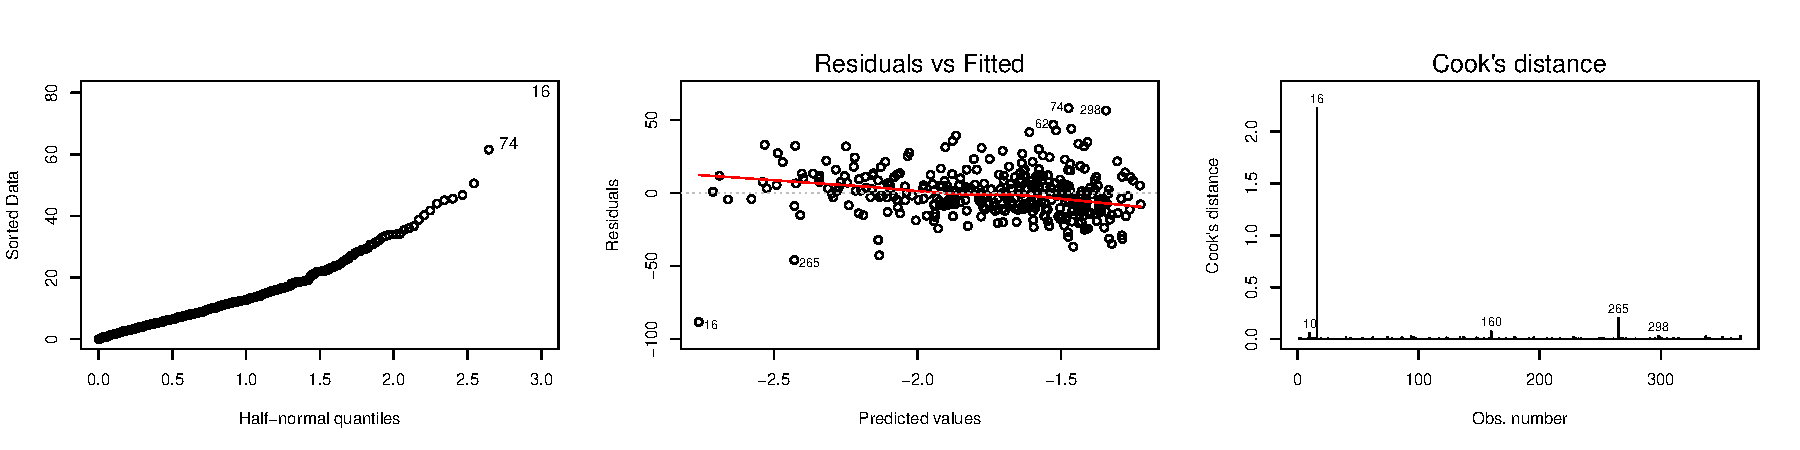
\includegraphics{Report_files/figure-latex/unnamed-chunk-16-1} 

}

\caption{\label{ass_mdl2}Diagnostics first quasi-binomial model}\label{fig:unnamed-chunk-16}
\end{figure}

The left plot of figure \ref{ass_mdl2} visualizes the half-normal
quantiles against the pearson residuals. Ideally, these residuals would
not be greater than 3. However, this plot shows residuals even up to 80.
The middle plot displays the predicted values against the deviance
resiuals. Also here a large spread of the residuals is observed and the
variance tends to increase with an increase of the fitted value. The
right plots visualizes the cook's distance, which can identify
influential observations. Observation 16 is an outlier, because it is
very influential and stands out from any pattern in the residual plots.
Furthermore, Dinkelland (obs 74) and Rotterdam (obs 265) are also
influential. Amsterdam is the municipality with the lowest percentage of
CDA votes and Dinkelland has the highest percentage of CDA votes.

\begin{figure}[H]

{\centering 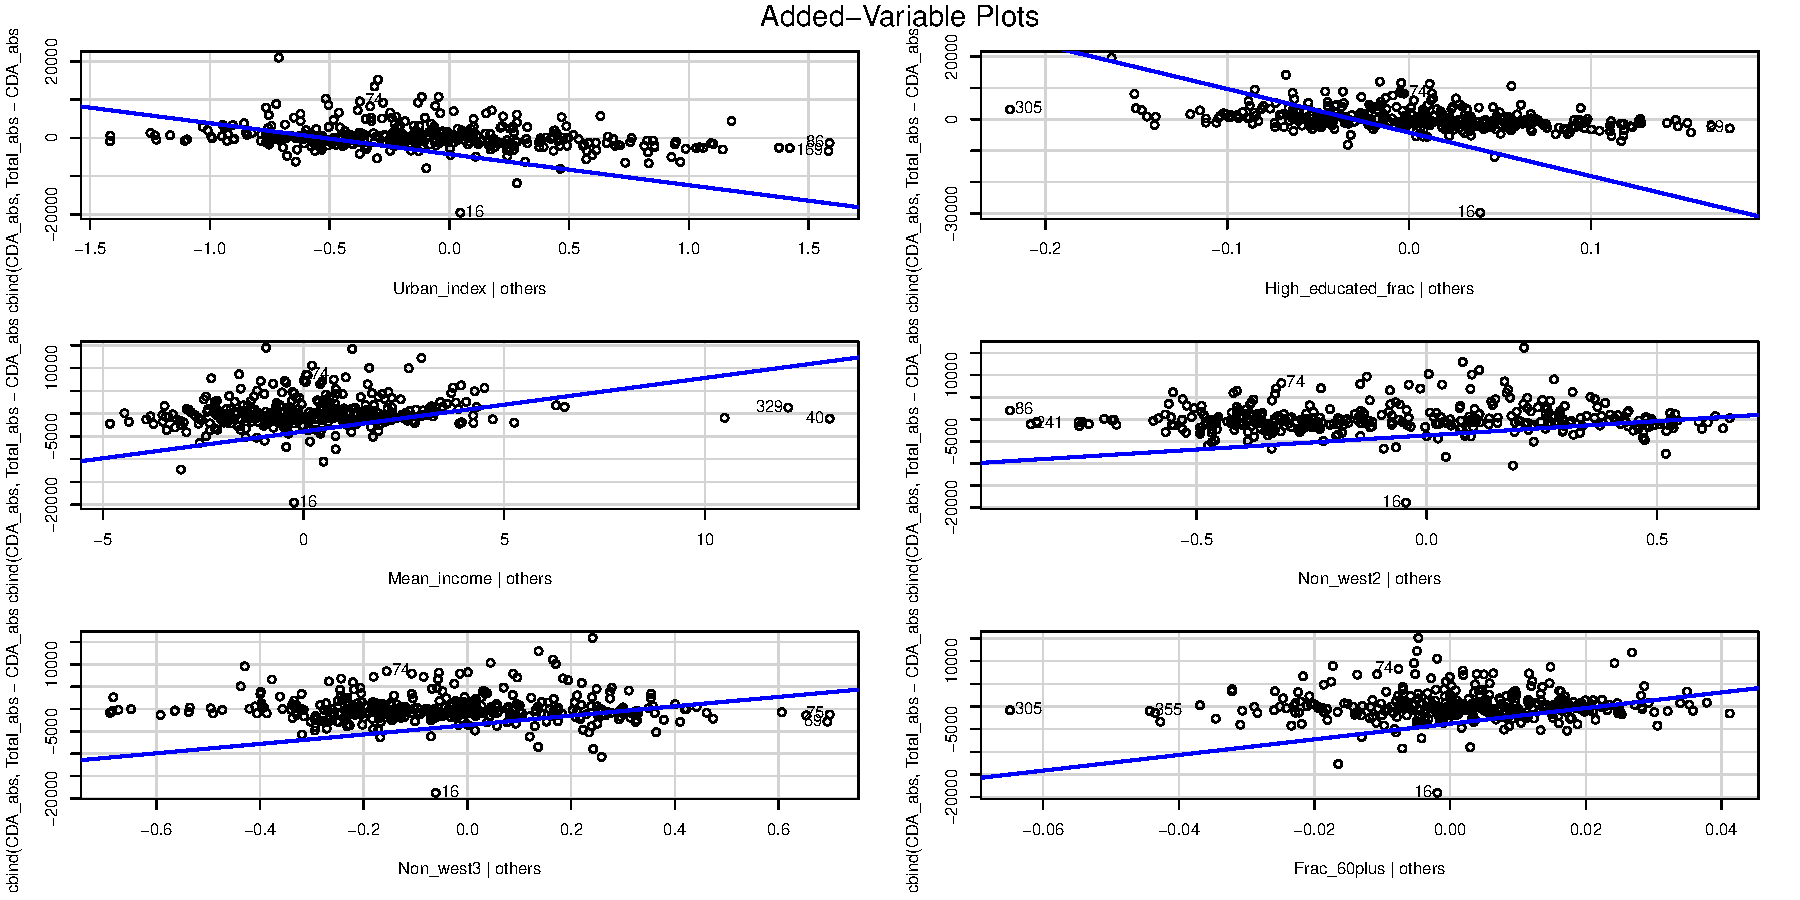
\includegraphics{Report_files/figure-latex/unnamed-chunk-17-1} 

}

\caption{\label{av_mdl2}AvPlots first quasi-binomial model}\label{fig:unnamed-chunk-17}
\end{figure}

Figure \ref{av_mdl2} help to interpret the partial regression
coefficients in a model when the other variables are held constant. The
partial regression line is highly influenced by observation 16 again.
The blue lines do not represent the data well at the moment.

\subsection{3.3 Third model}\label{third-model}

For this model the variable \texttt{Frac\_60plus} is removed, because it
had the lowest F-value. Furthermore, the observations 16 (Amsterdam) and
265 (Dinkelland) are removed. These influence the partial regression
coefficients greatly and have large residuals and cook's distances.
These steps were originally done in two, but are combined for this
report.

Below the summary output from this third model:

\begin{table}[ht]
\centering
\begin{tabular}{rrrrr}
  \hline
 & Estimate & Std. Error & t value & Pr($>$$|$t$|$) \\ 
  \hline
(Intercept) & -1.0878 & 0.1802 & -6.04 & 0.0000 \\ 
  Urban\_index & -0.1352 & 0.0303 & -4.46 & 0.0000 \\ 
  High\_educated\_frac & -1.2202 & 0.3126 & -3.90 & 0.0001 \\ 
  Mean\_income & -0.0004 & 0.0082 & -0.05 & 0.9583 \\ 
  Non\_west2 & -0.1232 & 0.0479 & -2.57 & 0.0105 \\ 
  Non\_west3 & -0.3447 & 0.0691 & -4.99 & 0.0000 \\ 
   \hline
\end{tabular}
\end{table}

By removing observation 16 and 265, the factor \texttt{Non\_west2} has
become significant. The null deviance has dropped to 173,842 with 363 df
and the residual deviance has decreased slightly to 76,966 with 358 df.
\(\phi\) has increased slightly to 221.709.

\begin{figure}[H]

{\centering 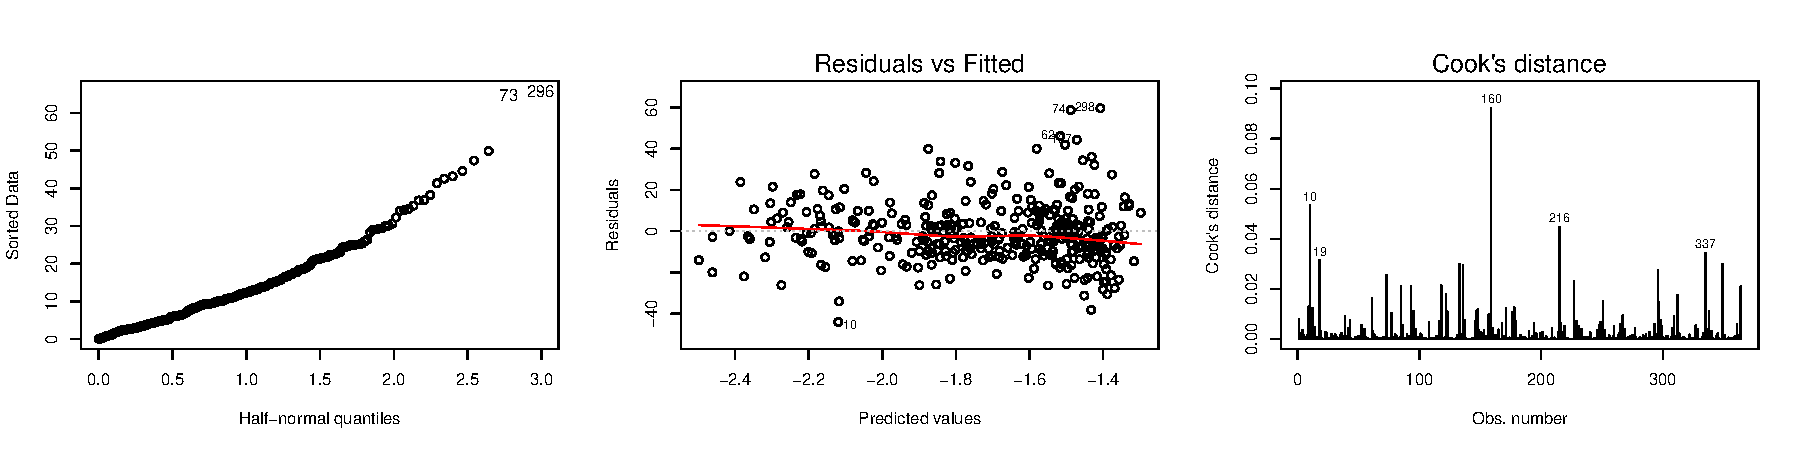
\includegraphics{Report_files/figure-latex/unnamed-chunk-19-1} 

}

\caption{\label{ass_mdl3}Diagnostics third quasi-binomial model}\label{fig:unnamed-chunk-19}
\end{figure}

The plot left still displays very large pearson residuals. The plot in
the middle still visualized that the deviance residuals tend to increase
when the predicted values increase. The cook's distance no longer
displays highly influential observations.

\begin{verbatim}
## Single term deletions
## 
## Model:
## cbind(CDA_abs, Total_abs - CDA_abs) ~ Urban_index + High_educated_frac + 
##     Mean_income + Non_west
##                    Df Deviance F value    Pr(>F)    
## <none>                   76966                      
## Urban_index         1    81396 20.6048 7.721e-06 ***
## High_educated_frac  1    80361 15.7942 8.543e-05 ***
## Mean_income         1    76966  0.0028    0.9577    
## Non_west            2    82994 14.0208 1.373e-06 ***
## ---
## Signif. codes:  0 '***' 0.001 '**' 0.01 '*' 0.05 '.' 0.1 ' ' 1
\end{verbatim}

According to the F-test \texttt{Mean\_income} should be removed as well,
because the F-value is below 1 and the corresponding p-value is 0.96.

\subsection{3.4 Final model}\label{final-model-1}

The final model is reached after dropping the variable
\texttt{Mean\_income}. It's formula is as follows:

\(logit(\theta_{i}) = -1.09 -0.13 \cdot UrbanIndex -1.23 \cdot HighlyEducatedFraction - 0.12 \cdot NonWest:2 - 0.34 \cdot NonWest:3 + \epsilon_i\)

The summary output is as follows:

\begin{table}[ht]
\centering
\begin{tabular}{rrrrr}
  \hline
 & Estimate & Std. Error & t value & Pr($>$$|$t$|$) \\ 
  \hline
(Intercept) & -1.0965 & 0.0653 & -16.80 & 0.0000 \\ 
  Urban\_index & -0.1350 & 0.0300 & -4.50 & 0.0000 \\ 
  High\_educated\_frac & -1.2297 & 0.2541 & -4.84 & 0.0000 \\ 
  Non\_west2 & -0.1235 & 0.0477 & -2.59 & 0.0100 \\ 
  Non\_west3 & -0.3444 & 0.0688 & -5.01 & 0.0000 \\ 
   \hline
\end{tabular}
\end{table}

\begin{verbatim}
## Single term deletions
## 
## Model:
## cbind(CDA_abs, Total_abs - CDA_abs) ~ Urban_index + High_educated_frac + 
##     Non_west
##                    Df Deviance F value    Pr(>F)    
## <none>                   76966                      
## Urban_index         1    81471  21.009 6.318e-06 ***
## High_educated_frac  1    82190  24.364 1.223e-06 ***
## Non_west            2    83077  14.251 1.108e-06 ***
## ---
## Signif. codes:  0 '***' 0.001 '**' 0.01 '*' 0.05 '.' 0.1 ' ' 1
\end{verbatim}

According to the F-test all variables now significantly contribute to
the model. The null deviance is still 173,842 with 363 df and the
residual deviance has slightly decreased to 76,966 with 359 df. \(\phi\)
is estimated at 221.1.

\begin{figure}[H]

{\centering 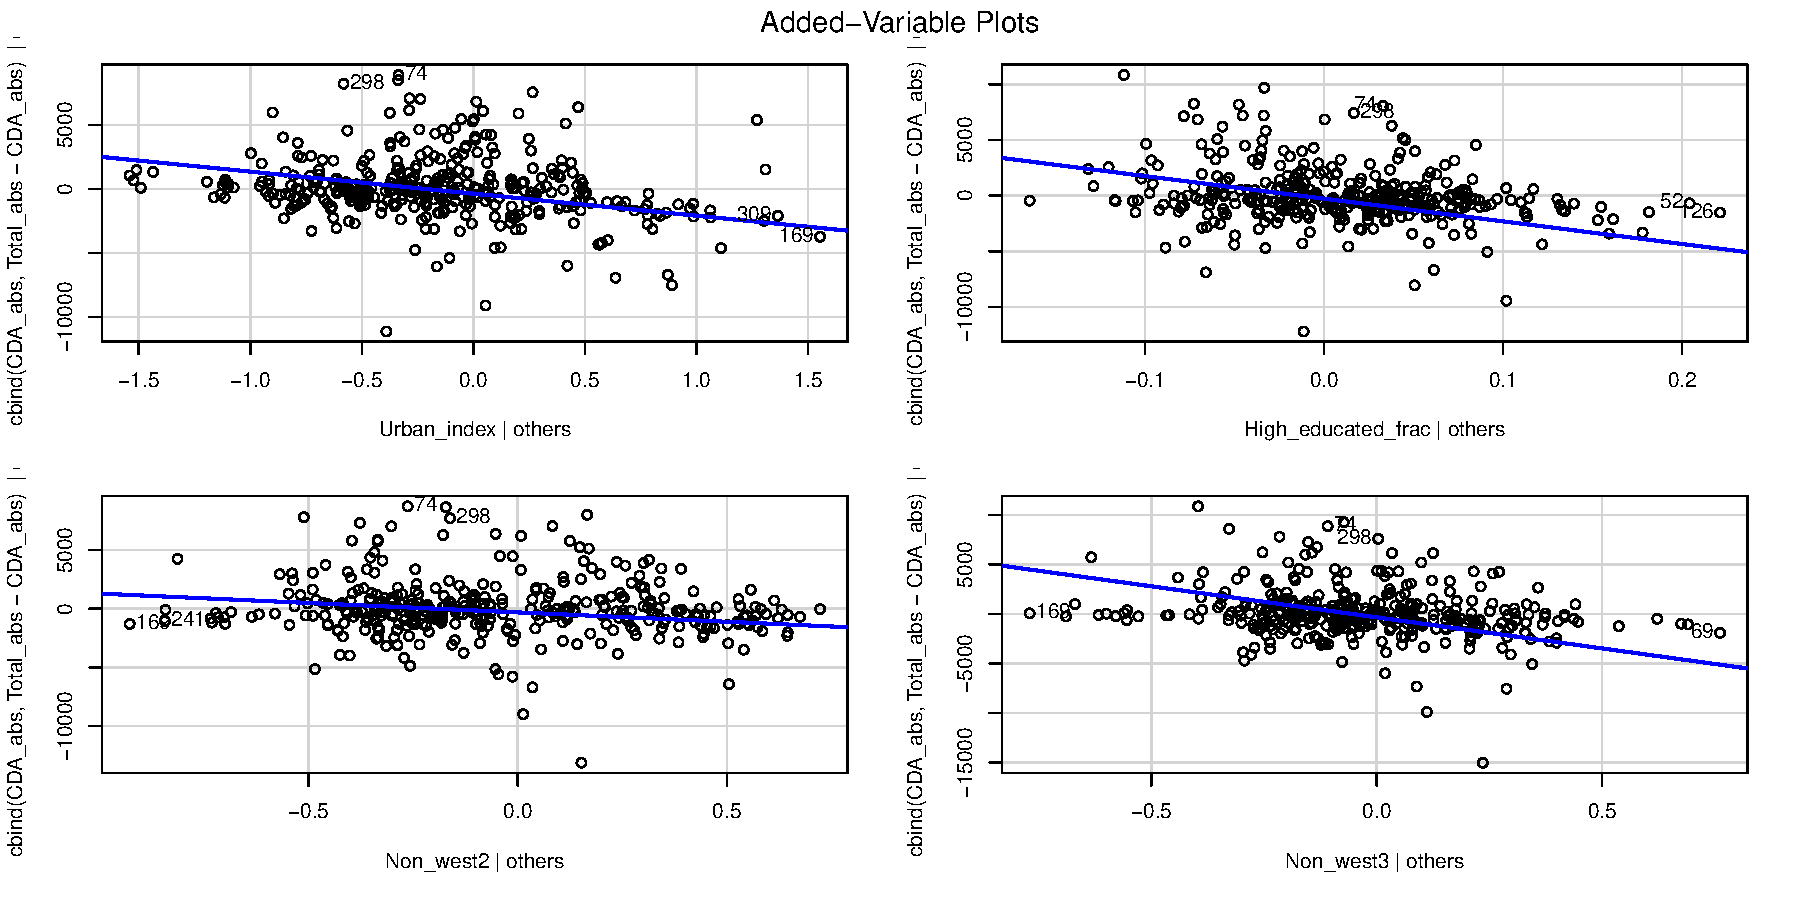
\includegraphics{Report_files/figure-latex/unnamed-chunk-22-1} 

}

\caption{\label{ass_final}Diagnostics final quasi-binomial model}\label{fig:unnamed-chunk-22}
\end{figure}

Figure \ref{ass_final} displays that there is still a large spread of
both the pearson (left plot) and deviance (middle plot) residuals.
Furthermore, there is non-constant errror variance. The cook's distance
does not display very influential observations.

\begin{figure}[H]

{\centering 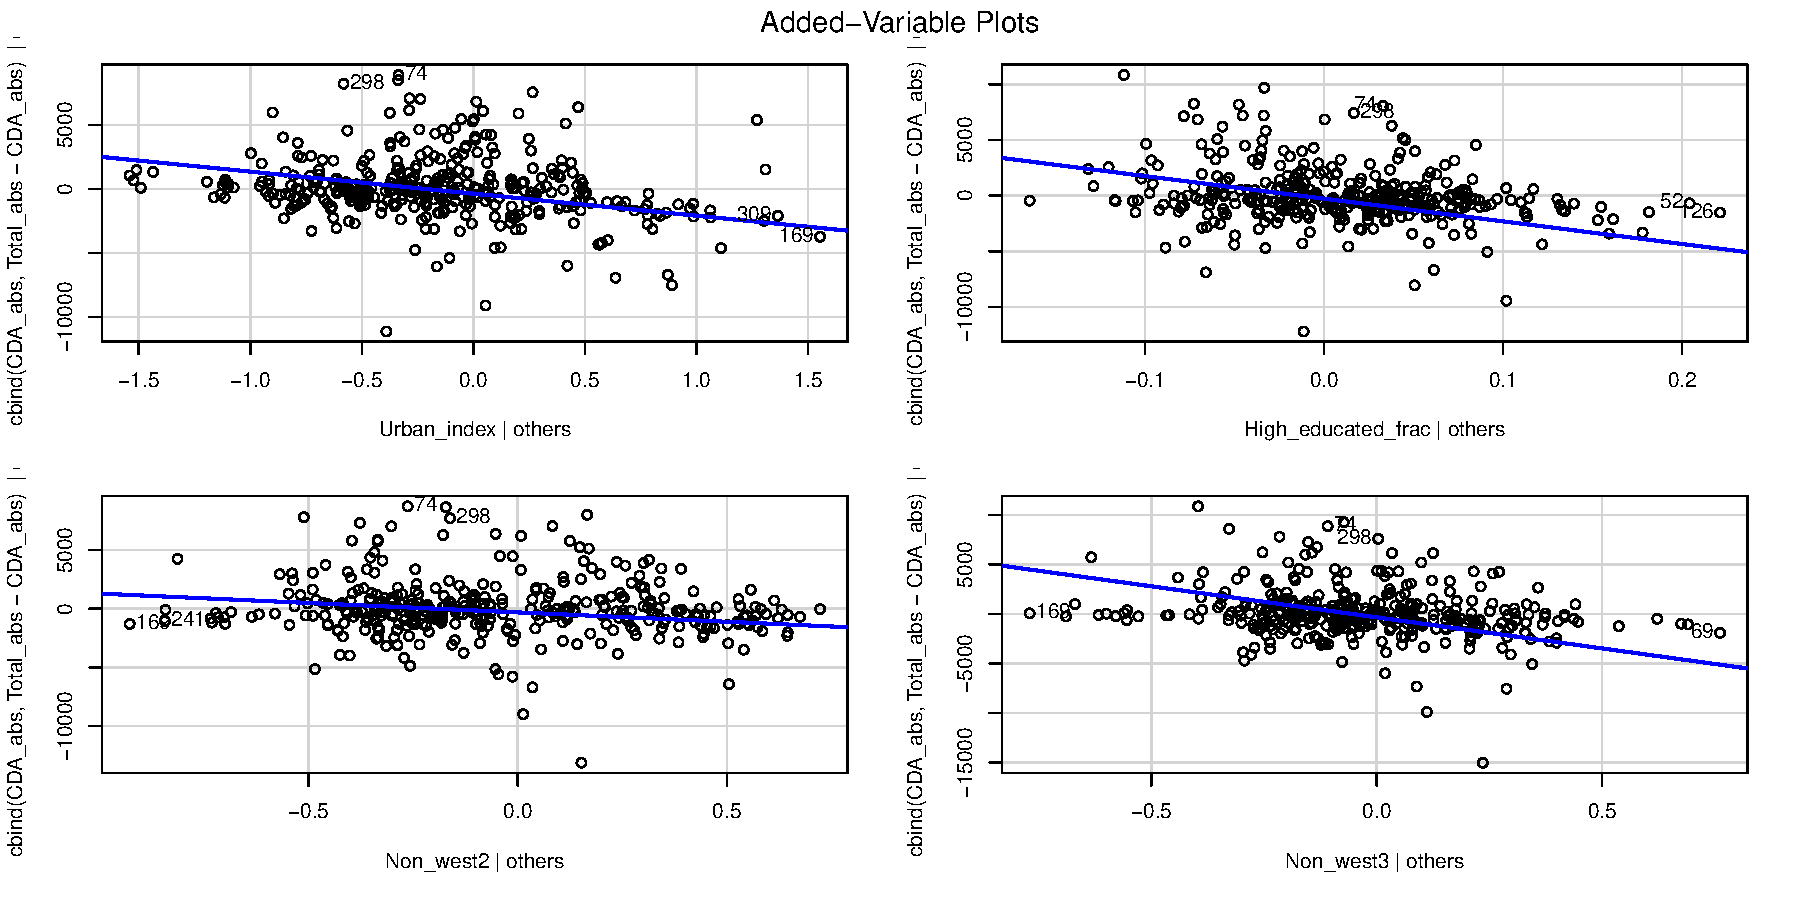
\includegraphics{Report_files/figure-latex/unnamed-chunk-23-1} 

}

\caption{\label{av_final}Diagnostics final quasi-binomial model}\label{fig:unnamed-chunk-23}
\end{figure}

\begin{verbatim}
##        Urban_index High_educated_frac          Non_west2 
##       0.0012896670       0.0004230904       0.0007928046 
##          Non_west3 
##       0.0012734699
\end{verbatim}

After removing two outliers, the partial regression coefficients
represent the data much better. There are no strong correlations between
the explanatory variables and the respons. The low VIF values also
indicate this.

\subsection{3.5 Cross validation}\label{cross-validation-1}

At last, the logistic model is validated by k-fold validation. This
dataset has 366 observations, therefore K = 5 is enough. The code for
cross validation is similar to the one used for the linear model.
Therefore, only the output is presented here and not the code.

\begin{verbatim}
##  1  2  3  4  5 
## 74 73 73 73 73
\end{verbatim}

\begin{verbatim}
## [1] 0.001708063
\end{verbatim}

The cross validation results in a Means Squared Error (MSE) of 0.0017.

\subsection{Discussion}\label{discussion}

\subsection{Linear regression}\label{linear-regression}

Because the fitted values are transformed to a ln form, it is also
possible to raise the coëfficients to a exponential power. The final
model obtained then is:

\(Y_i = e^(-1.0298 -0.8277*high educated fraction -0.1311*Urban index -0.1141*Non west2 -0.2871*Non west3 -3.0168*Frac 60plus + \epsilon i)\)

Per variable the influence will be discussed. The slope will start at
point exp(-1.0298), this is equal to 0.357. This means if all the other
demographic variables are zero, the fitted value will be equal to the
intercept, so equal to 0.357. This not a possible outcome, because a
Municipality with all these demographics equal to zero is no reality.
For the other coefficients it is a bit harder to predict there
influence, because of the log transformation and the different range the
different variables have. For example, the urban index has a 0-3.8 range
and education ahs a 0.12-0.47 range in this data set. But still some
remarks can be made about the slope of the model. The fraction 60 plus
has the lowest marginal impact on the slope, if everything else stays
the same an frac 60 plus changes for example 1 the exponent changes with
-3.02. The non west2 has the highest impact on the slope, because the
coëfficient is the lowest. Another important point is that or Non-west2
and Non-west3 are both zero, or Non-west2 is one ore Non west 3 is one.
The outcome of the crossvalidation for this model is 0.0582. So the mean
squared difference between the fitted and predicted value is 0.0582,
which is pretty close to 0.

There are some limitations for this model, because the response variable
is a fraction and will never be larger than one, theoratically a
Generalized linear model would be better. Also some assumptions are
violated. In the fitted vs residual graph it is visible that the
variance is not equally spread, there is a small ``loudspeaker
pattern''. But because the fitted values are log transformed, it is not
really possible to adapt this any further. Also there are two
municipalities that fall outside the {[}-3,3{]} range in the normality
plot, but because they are still in the 95\% envelope the decision is
made to not delete these municipalities.

\subsection{Further research}\label{further-research}

Both of the models have different significant variables. But it is
difficult to say which one is a better fitting model. Because both of
them have reasons to choose that kind of model, also both of them have
limitations. That is why further research should be done to research
which of the model is the best fitting model. Another topic that can be
researched in further research is the influence of demographics on areas
of municipalities instead of whole municipialities. Because differences
between areas are nullified in the demographics of a municipality.

\subsection{4.2 Logistic regression}\label{logistic-regression-1}

For the final model two variables and two outliers are removed. The
coefficients of the model are on the log-odds scale and need to be
transformed before interpretating them. Each estimated coefficient is
the expected change in the log odds of voting for CDA for a unit
increase in the corresponding explanatory variable holding the other
explanatory variables constant.

The coefficient for \emph{Urban Index} is the difference in the log
odds. In other words, the expected change in log odds of voting for CDA
is -0.13. This can be transformed to the odds: \(exp(-0.13)\) = 0.88.
The odds of voting for CDA decrease with roughly 12\% if the Urbanity
increases with one unit. The Urbanity index has a range from 0 to 4, so
this variable has a large influence. For example, when comparing
Terschelling (Urbanity index of 0) and Leiden (Urbanity index of 3.7),
the expected decrease is 40.7\%.

An similar calculation can be done for one unit increase of \emph{Non
west}. When \emph{Non west} increases from 1 (the reference level) to 2
and the other explanatory variables are held constant, then the log odds
of voting for CDA is -0.12. Transforming this to the odds results in a
decrease of 11\%, roughly. And when when comparing factor level 1 to 3,
the log odds is -0.34. This results in the odds of \(exp(-0.34)\) =
0.71, a decrease of 29\%. This is not a simple duplication of level 2.

According to the model, holding \emph{Highly educated} and \emph{Non
west} constant, the odds of voting for CDA if the Urban index increases
with 1 unit is \(exp(-0.16)\) = 0.87. In percentage change does this
mean that the odds decrease with 12.6\%.

At last, the odds of voting for CDA if \emph{Highly educated} increases
with 1 unit is \(exp(-1.23)\) = 0.29. In percentage change does this
mean that the odds decrease with 70.8\%. This is a very large decrease,
but can be explained. This variable is a fraction and has a range from 0
- 1. An increase of one unit is not likely to happen.

In summary, municipalities in rural areas, with smaller amounts of
Non-western and Highly educated residents tend to vote for CDA. Below
the formula with the odds ratio is shown:

\(\frac{\theta_i}{1 - \theta_i}) = 0.33 + 0.88 \cdot UrbanIndex + 0.29 \cdot HighlyEducatedFraction - 0.89 \cdot NonWest:2 + 0.71 \cdot NonWest:3 + \epsilon_i\)

As already said, there is still dispersion, even after using a quasi
binomial model. A possible explanation can be clustering of
observations. Municipalities close to each other will probably vote
similar. Figure \ref{Results elections} shows that the municipalites
where CDA (shown in light green) is the biggest party are clustered
together. CDA is the biggest party in large parts of Friesland,
Groningen and Drente. The municipalities located here are probably have
a similar population.

\begin{figure}
\centering
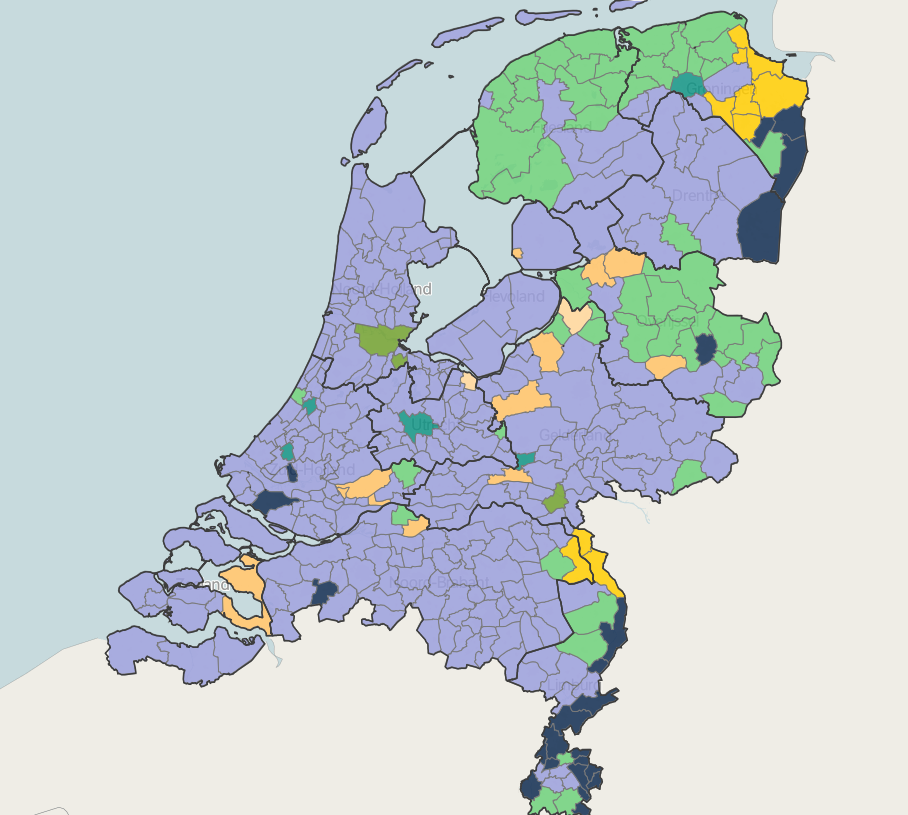
\includegraphics[width=2.60417in]{Uitslag_verkiezingen2017.png}
\caption{Results elections with biggest parties. CDA is displayed in
light green}
\end{figure}

Another explanation for the dispersion is the large variation. In some
municipalities only 3\% voted for CDA, while in other almost 50\%. This
large variation is hard to modeled in a binomial. By using the log odds,
votes are distributed in two groups: voted for CDA or not voted for CDA.
However, with 13 political parties is it hard to distinguish two groups.
Because it is not possible to into account which parties are similar to
CDA.

Even though, the cross validation resulted in a MSE of 0.0017, it is not
likely that this model can make future predictions. This because of the
large variation and overdispersion.

\section{5. Conclusion}\label{conclusion}

-samenvatting -belangrijkste limitaties noemen -modellen met elkaar
vergelijken


\end{document}
